%Nama Kelompok 1				
%Kelas D4 TI 1B							
%ADAM NOER HIDAYATULLAH 1174096 
%SAVA REYHANO 1174046
%FAISAL NAJIB A 1174042
%MOHAMMAD ATHALLARIQ FATHURAMADHANDI P. B  1174055
%IHSAN KAMAL BANGUN  1174045
%MUHAMAD LAZUARDI HABIBILLAH RITONGA 1174061
%RESTIYANA DWI ASTUTI (1154077)
	\section{Definisi Arsitektur Komputer}
	Tentang Komputer,pada gambar ini\ref{komputermodern} merupakan struktur dari sebuah komputer modern.Namun komputer ini berawal dari.... 
	Komputer berasal dari bahasa latin Computare yang berarti menghitung(to compute), karena pada awalnya komputer pertama yang dirancang digunakan untuk keperluan perhitungan. 
	Inspirasinya diambil dari alat hitung tertua yaitu bernama \'Abaccus\'(SM 300) atau lebih dikenal dengn sipoa yang berasal dari negeri cina.
	Konsep komputer yang pertama kali dirancang oleh Howard G.Aitiken,seorang doktor dari Harvard University (1937),bekerja sama dengan IBM (International Business Machine Corp). 
	Yang berhasil membuat sebuah mesin yang bekerja dengan tenaga elektromagnetik yang diberi nama Harvard Mark-1. 
	Komputer pertama di muka bumi ini mempunyai berat setaras sapi yaitu 5 ton dan memiliki kemampuan kalkulassi selama 6 detik mencapai angka 23 digit.
	ENIAC pada tahun 1942 (dengan sistem binari digit 8bit dan memori),pernah diakui sebagai komputer pertama. 
	Akhir-akhir ini diketahui juga bahwa Konrad Zuse dari jerman pada tahun 1941 sudah membuat mesin \'komputer\' yang dapat diprogram dan bekerja menggunakan sistem biner. 
	Namun karena jerman kala itu masih terisolasi saat perang dunia 2, maka ENIAC tetap diakui sebagai 
	komputer pertama yang memakai prinsip digital dengan sistem memori dan binari digit (8bit)
	Komputer pribadi (PC) pertama yang dikembangkan oleh Ed Roberts,yaitu Altair 8800 diluncurkan melalui promo majalah Popular Electronics di bulan januari 1975.
	Altair 8800 sebetulnya sebuah kit yang dirakit menjadi \'MESIN KOMPUTER\'. 
	Pada saat itu yang namanya komputer adalah mainframe yang ukurannya raksasa dan harganya jutaan dolar sehingga kit buatan MITS (Microinstrumentation and TelementrySystems,Albuqurerque,New Mexico USA) yang dijual seharga sekitar US\$400 mendapat penggemar yang cukup banyak.
	Padahal \'Komputer\' ini tidak memiliki keyboard, screen, ataupun printer. 
	Switch Yang ada kala itu dapat digunakan untuk memasukkan bilangan biner dan outputnya menunjukkan LED yang menyala untuk.
	Kit Altair 8800 ini lebih populer ketika William Gates (Bill Gates yang dilahirkan di seattle tanggal 28 Oktober 1955) mengembangkan bahasa BASIC untuk \'Komputer\' Altair ini. 
	Banyak orang pada awalnya menyangsikan bahwa,bahasa BASIC tidak akan mampu dimasukkan ke dalam \'komputer\' ini. 
	Namun Bill Gates membuktikan hal itu bisa dilakukan, setelah penciptaan keyboard dan monitor tentunya. 
	Bill Gates adalah Chairman and Chief Executive Officer(CEO) dari microsoft Corporation,yang didirikannya di tahn 1975.
	Kini dengan pengatahuan dan pengalamannya, dia merupakan salah satu dari orang terkaya di dunia.\cite{syafrizal2005pengantar}
	\begin{figure}[ht]
		\centerline{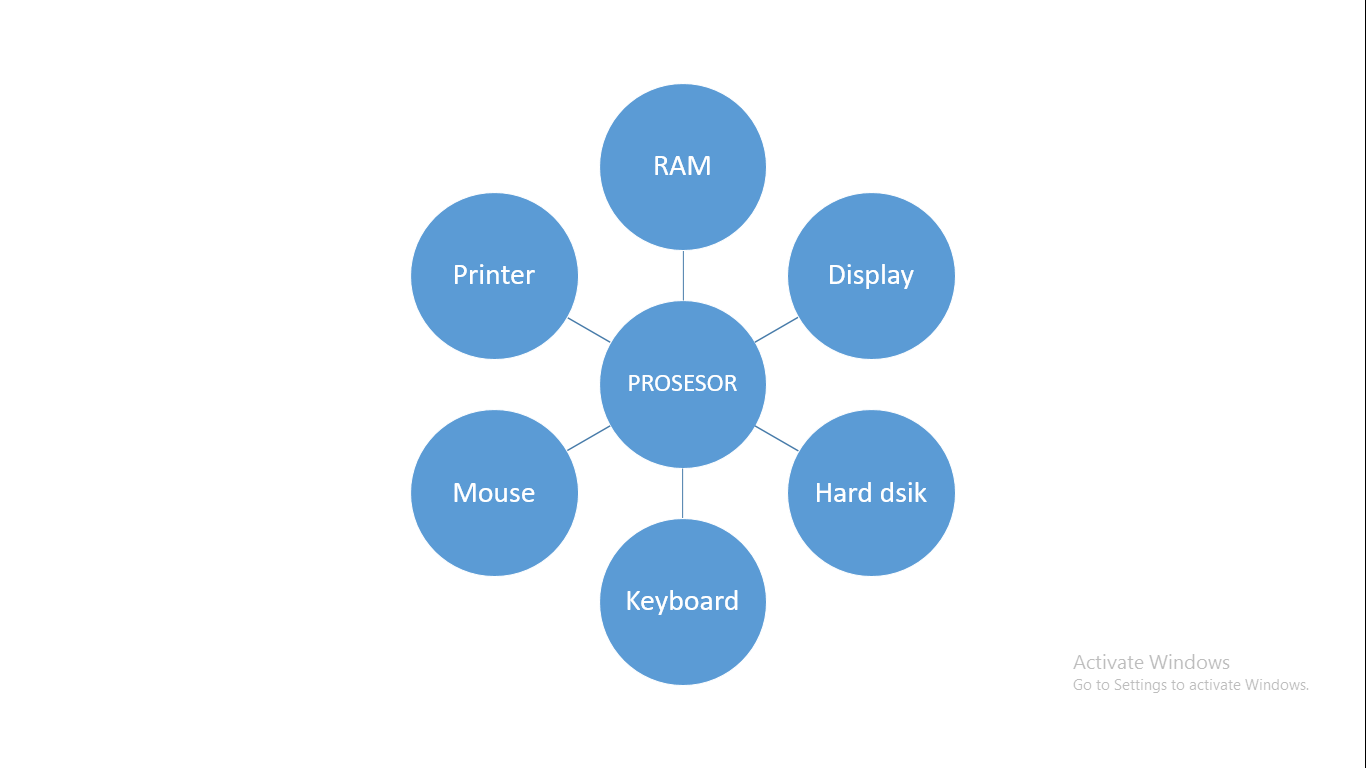
\includegraphics[width=1\textwidth]{figures/komputermodern.png}}
		\caption{Merupakan struktur dari sebuah mesin Komputer/Hardware untuk menggunakan Komputer.}
		\label{komputermodern}
	\end{figure}
	
	\subsection{Sejarah}
Arsitektur komputer terdokumentasi pertama ada dalam korespondensi antara Charles Babbage dan Ada Lovelace, yang menggambarkan mesin analitis. Saat membangun komputer Z1 pada tahun 1936, Konrad Zuse menjelaskan dalam dua aplikasi paten untuk proyek masa depannya bahwa instruksi mesin dapat disimpan dalam penyimpanan yang sama yang digunakan untuk data, yaitu konsep program tersimpan. \cite{faberkonrad} Dua contoh awal dan penting lainnya adalah:
\begin{itemize}
\item Makalah karya John von Neumann tahun 1945, Draft Pertama Laporan tentang EDVAC, yang menggambarkan sebuah organisasi elemen logis; \cite{von1945first}
\item Kalkulator Elektronik Kalkulator Alan Turing yang lebih rinci untuk Mesin Komputasi Otomatis, juga 1945 dan yang mengutip makalah John von Neumann. \cite{copeland2005alan}
\end{itemize}

Istilah \"arsitektur\" dalam literatur komputer dapat dilacak pada karya Lyle R. Johnson, Frederick P. Brooks, Jr., dan Mohammad Usman Khan, semua anggota departemen Organisasi Mesin di pusat penelitian utama IBM pada tahun 1959. Johnson telah kesempatan untuk menulis sebuah komunikasi riset eksklusif tentang Stretch, sebuah superkomputer yang dikembangkan IBM untuk Laboratorium Nasional Los Alamos (yang saat ini dikenal sebagai Laboratorium Ilmiah Los Alamos). Untuk menggambarkan tingkat detail untuk membahas komputer mewah, dia mencatat bahwa deskripsi format, jenis instruksi, parameter perangkat keras, dan perangkat tambahan kecepatannya berada pada tingkat \"arsitektur sistem\" - istilah yang nampaknya lebih berguna daripada \"organisasi mesin.\"
Arsitektur komputer, seperti arsitektur lainnya, adalah seni untuk menentukan kebutuhan pengguna suatu struktur dan kemudian merancang untuk memenuhi kebutuhan tersebut seefektif mungkin dalam batasan ekonomi dan teknologi.
Brooks melanjutkan untuk membantu mengembangkan IBM System / 360 (sekarang disebut IBM zSeries) baris komputer, di mana \"arsitektur\" menjadi kata benda yang mendefinisikan \"apa yang pengguna perlu ketahui\". Kemudian, pengguna komputer menggunakan istilah ini dengan banyak cara yang kurang eksplisit. \cite{hellige2004genese}
Arsitektur komputer paling awal dirancang di atas kertas dan kemudian langsung dibangun ke dalam bentuk perangkat keras terakhir. \cite{copeland2005alan} Kemudian, prototip arsitektur komputer secara fisik dibangun dalam bentuk komputer logika transistor-transistor (TTL) - seperti prototip dari 6800 dan PA-RISC yang diuji, dan di-tweak, sebelum melakukan sampai pada bentuk perangkat keras terakhir. Pada tahun 1990an, arsitektur komputer baru biasanya \"dibangun\", diuji, dan di-tweak-di dalam beberapa arsitektur komputer lainnya di simulator arsitektur komputer; atau di dalam FPGA sebagai mikroprosesor yang lembut; atau keduanya-sebelum melakukan ke bentuk perangkat keras terakhir. \cite{hellige2004genese}
	\subsection{Pembahasan Arkom}
	\subsection{Survey dari Pararel Arsitektur Komputer}
	Sebuah usaha dibuat untuk mengganti inovasi arsitektur terbaru,dengan konteks pengembangan arsitektur parael yang lebih luas dengan menyurvei fundamental arsitektur komputer dari yang lebih baru dan lebih mapan dan dengan menempatkan alternatif arsitektur ini dengan kerangka kerja yang koheren.
	Penekanan utama adalah pada konstruksi arsitektural daripada mesin paralel yang spesifik.
	Tiga kategori arsitektur yang didefinisikan dan didiskusikan: arsitektur sinkron, terdiri dari vektor, SIMD (single-instruction-stream, multiple-data-stream) dan mesin sistolik; MIMD (multiple-instruction-stream, multiple-data-stream) dengan memori terdistribusi atau shared; dan paradigma berbasis MIMD, terdiri dari tipe hibrida MIMD / SIMD, dataflow, reduction, dan wavei.\cite{duncan1990survey}

	\subsection{Pengurangan Instruksi Instruksi Komputer untuk VLSI}

	Sirkuit terintregasi menawarkan implementasi sistem digital yang kompak dan murah dan menyediakan perfoma melalui keuntungan. 
	Komunikasi on-chip bandwidth tinggi terhadap mereka.saat ini teknologi sedang di gunakan membuat tujuan umum von Neumann processor. 
	Sebaiknya integrasikan sebanyak mungkin mengunakan fungsi pada satu chip, sehingga meminimalkan komunikasi off-chip.
	Bahkan dalam sirkuit Large Scale Integrated (VLSI), transistor yang tersedia di area chip terbatas merupakan sumber daya langka saat digunakan untuk implementasi prosesor atau bahkan komputer yang lengkap, dan karenanya, penggunaannya harus efektif.
	Disertasi ini menunjukkan bahwa tren baru dalam arsitektur komputer terhadap rangkaian instruksi peningkatan kompleksitas menyebabkan penggunaan sumber daya langka yang tidak efisien.
	Kami menyelidiki alternatif arsitektur Computer Instruction Instruction Set (RISC) yang memungkinkan penggunaan transistor on-chip secara efektif dalam unit fungsional yang menyediakan akses cepat ke operan dan instruksi yang sering digunakan.
	Dalam disertasi ini, sifat perhitungan tujuan umum dipelajari, menunjukkan kesederhanaan operasi yang biasanya dilakukan dan frekuensi akses operan yang tinggi, banyak di antaranya dibuat pada beberapa variabel prosedur skalar lokal. 
	Arsitektur prosesor RISC I dan II dipresentasikan. Mereka menampilkan instruksi sederhana dan file register multi-jendela besar, yang jendela tumpang tindihnya digunakan untuk menyimpan argumen dan variabel skalar lokal dari prosedur yang paling baru diaktifkan. 
	Dalam kerangka proyek RISC, yang telah menjadi upaya tim besar di UC Berkeley selama lebih dari tiga tahun, sebuah prosesor single-chip RISC II nMOS dilaksanakan, bekerja sama dengan R. Sherburne. 
	Ersitekturrsitektur mikro-nya dijelaskan dan dievaluasi, diikuti dengan diskusi tentang metode debugging dan pengujian yang digunakan. Teknologi VLSI masa depan akan memungkinkan integrasi sistem yang lebih besar pada satu chip tunggal.
	Pemanfaatan yang efektif dari transistor tambahan dipertimbangkan, dan diusulkan agar digunakan dalam mengimplementasikan unit pengambilan dan urutan instruksi khusus yang terorganisir dan.
	Studi dan evaluasi arsitektur RISC II, serta disain, tata letak, dan pengujian setelah fabrikasi, telah menunjukkan kelayakan dan keuntungan dari pendekatan RISC. Prosesor single-chip RISC II terlihat berbeda dari prosesor komersil populer lainnya.
	transistor ini kurang total, hanya menghabiskan 10\% area chip untuk kontrol daripada satu setengah sampai dua pertiga, dan dibutuhkan desain kurang lebih lima kali lipat dan lay-out usaha untuk mendapatkan hasil yang hampir sempurna.\cite{katevenis1983reduced}

	\subsection{Pemodelan Kinerja Jaringan Komunikasi dan Arsitektur Komputer (Komputer Internasional)}

	Dalam kemajuan teknologi, kemampuan dalam berkomunikasi menjadi lebih rumit dengan kecepatan dan kapasitas yang semakin besar. 
	dengan semakin berkembangnya ilmu komunikasi, ini dapat membuat perkembangan kinerja arsitektur komputer semakin rumit karena harus dibandingkan 
	dengan kecepatan transfer.\cite{harrison1992performance}

	\subsection{MinneSPEC: Sebuah Benchmark SPEC SPEC untuk Proyek Simulasi Berbasis Arsitektur Komputer}

	Arsitektur komputer harus menetukan secara dengan benar mengunakan sumber komputasi yaitu algoritma yang di gunakan untuk menemukan suatu cara dalam memacahkan masalah dari sebuah data input
	Untuk menfasilitasi sebagai benchmarkprogram yang telah di kembangkan inputset MinneSPEC untuk rangkainya adalah benchmark SPEC CPU 2000 untuk beban kerjanya  memungkinkan arsitektur komputer mendapat hasil simulasi dengan waktu yang tepat.
	Ini ada tolak ukurnya  yang valid untuk penelitian berbasis simulasi. 
	Dalam proses pengembangan datasheet, MinneSPEC telah mengukur perhitungan,bentuk pola eksekusi tingkat fungsinya, dengan campuran instruksi,dan perilaku memori dibandingkan dengan program SPEC saat dijalankan dengan masukan referensi.\cite{kleinosowski2002minnespec}

	\subsection{Kebutuhan memori untuk arsitektur komputer yang seimbang}

	Salahlah satu dari akibatnya arsitektur komputer yang seimbang  adalah untuk menyeimbangkan linear rangkaian pe linear untuk melalukakn perhitungan matriks dan matriks trigulzisasi ukuran masing-masing memori lokal PE harus tumbuh secara linier.
	Jadi, semakin besar arraynya, semakin besar setiap memori lokal PE.\cite{kung1986memory}

	\subsection{Arsitektur komputer paralel untuk pemrosesan gambar}

	masalah pengolahan data melibatkan susunan data struktur cukup besar dan kebutuhan pengitungan sangat cepat skema pemrosesan pararel  kusus telah berevolusi selama 20 tahun 
	Sistem paralel yang telah dikembangkan untuk pengolahan citra digariskan dan fitur arsitektur.
	Sebagian besar arsitektur khusus dapat diklasifikasikan secara longgar seperti struktur SIMD atau pipa meskipun beberapa struktur MIMD telah dirancang untuk menganalisis citra tingkat yang  tinggi
	Dalam beberapa tahun terakhir beberapa skema multiple SIMD (MSIMD) telah diusulkan sebagai arsitektur yang sesuai untuk pemrosesan gambar.
	Pengembangan sistem MSIMD yang efektif dibahas dan model komputasi SIMD / MIMD.\cite{reeves1984parallel}

	\subsection{Blok berorientasi pengolahan operasi database relasional di arsitektur komputer modern}

	Sistem basis data tidak  akan sesuai untuk memanfaatkan arsitektur prosesor superscalar  yang modern Secara khusus, jam per instruksi (CPI) untuk query database yang agak sederhana cukup buruk dibandingkan dengan kernel ilmiah atau benchmark SPEC.
	Kurangnya kinerja sistem database disebabkan oleh rendahnya utilisasi cache dan unit fungsi prosesor serta hukuman percabangan yang lebih tinggi
	teknik pemrosesan yang berorientasi blok untuk evaluasi ekspresi agregasi dan operasi pemilahan sebagai fitur dalam sistem.\cite{padmanabhan2001block}

	\subsection{Arsitektur komputer RISC dikonfigurasi untuk meniru set instruksi komputer target}

	komputer arsitektur risc dikonfigurasi untuk meniru set intruksi komputer target untuk menjalankan perangkat lunak yang di tulis untuk komputer target, misalnya intel 80x86, motorola 680x0 atau mips R3000. 
	aparatus terintegrasi dengan komputer risc inti untuk membentuk komputer yang mengeksekusi intruksi risc yang di perluas.
	intruksi risc yang di perluas berisi bidang data yang menunjuk register tidak langsung yang mengarah ke register emulasi paling tidak sama dengan yang ada di komputer target. 
	namun, bidang dalam intruksi risc yang diperluas membatasi lebar yang ditiru dan dibutuhkan oleh intruksi yang ditiru tertentu.
	selain itu, intruksi risc yang diperluas berisi bidang yang menunjuk mode emulasi untuk kde kondisi dan memilih logika agar sesuai dengan kode kondisi komputer target. 
	intruksi target diurai dan dikirim ke urutan satu atau lebih intruksi risc yang diperluas untuk meniru setiap intruksi target.\cite{scantlin1996risc}

	\subsection{Database Arsitektur Komputer untuk Memanage sebuah program penghargaan dan mendapatkan pembayaran}

	Sistem distribusi informasi yang canggaih termasuk ke dalam jalur komunikasi yang mempunyai beberapa switching komunikasi selektif. 
	Hal itu menentukan apakah transaksi elektronik tersebut layak diterima atau tidak.
	Sistem komputer,yang intensif dapat mencakup titik sistem pengolahan yang menghasilkan laporan yang baik sesuai dengan kriteria yang di setujui.\cite{robinson1998database}

	\subsection{Arsitektur komputer berkinerja tinggi}

	Sebagian besar aktivitas perancangan komputer telah beralih ke komputer desain berkinerja tinggi,karena komputer desktop single-user mencapai titik pengiriman daya komputer lebih banyak dari pada mainframe yang lama.
	Karena akan lebih mudah untuk Topik yang dibahas meliputi: Pendekatan arsitektur umum seperti desain memori, teknik pipa, dan struktur paralel. 
	kemacetan mendasar seperti bandwidth memori, bandwidth proses, komunikasi, dan sinkronisasi, teknik evaluasi, contoh aplikasi nyata dan persyaratan arsitekturalnya.\cite{stone1987high}

	\subsection{Ifrastruktur untuk pemodelan sistem komputer}

	Perangcang dapat menjalankan program pemodelan perangkat, model perangkat lunak untuk memvalidasi kinerja dan ketepatan desain perangkat keras.
	pemrogram dapat menggunakan model  untuk mengembangkan dan menguji perangkat lunak sebelum perangkat keras sebenarnya tersedia.
	Tiga persyaratan penting mendorong penerapan model perangkat lunak: kinerja, fleksibilitas, dan detail. 
	Kinerja menentukan jumlah beban kerja yang dapat dilakukan model mengingat sumber daya mesin tersedia untuk simulasi.
	perangkat simplecar memiliki sebuah infrastruktur simulasi dan pemodelan arsitektural.
	Simulator SimpleScalar mereproduksi operasi sebuah  perangkat komputer dengan menjalankan instruksi program menggunakan penerjemah.
	instruktur instruksi telah mendukung :instruksi populer,termasuk alpha,PPC, x86, dan ARM.\cite{austin2002simplescalar}
	Bagian bagian arsitektur komputer
	Ini merupakan bagian-bagian arsitektur komputer\ref{sasasa}
		1 Software - perangkat lunak yang menjalankan hardware
		2 kernell - jembatan antara software dengan hardware
		3 Hardware - perangkat keras untuk menjalankan operasi komputer
    \begin{figure}[ht]
		\centerline{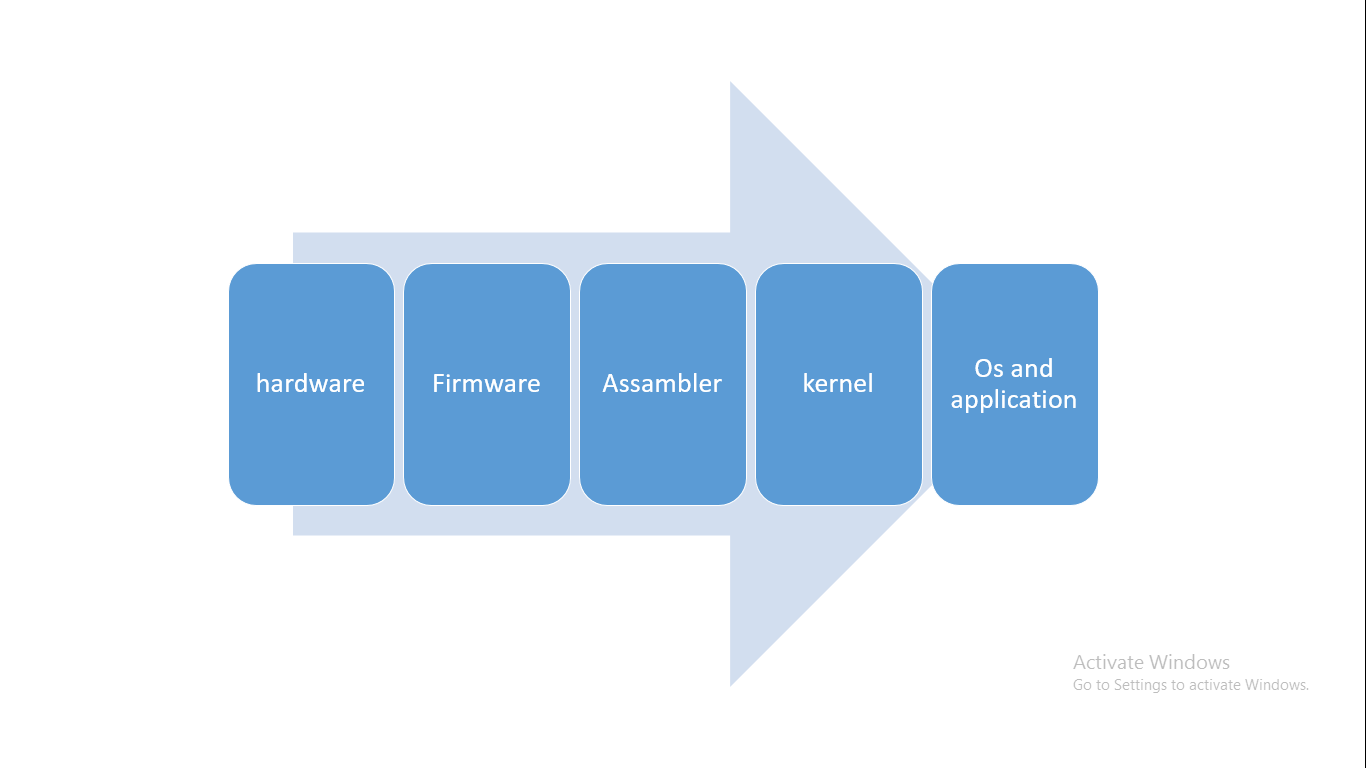
\includegraphics[width=1\textwidth]{figures/sasasa.PNG}}
		\caption{Bagian dari Arsitektur Komputer}
		\label{sasasa}
	\end{figure}
	
	\subsubsection{PENUTUP}
	\subsubsection{Fungsi dari Arsitektur Komputer}
	Sebuah tolak ukur untuk mengevaluasi Arsitektur Komputer berkinerja tinggi pada aplikasi Bioinformatika.
	Pertumbuhan eksponensia telah mendorong minat yang meningkat dalam informasi genetika berskala besar. 
	aplikasi bioinformatika, adalah aplikasi untuk memudahkan peneliti menyaring data data biologis secara besar besaran dan untuk mengekstrak informasi yang berguna, menjadi beban komputer yang semakin penting.
	Aplikasi tersebut sebagai perwakilan untuk perancangan dan evaluasi arsitektur komputer berkinerja tinggi untuk beban kerja yang muncul pada saat ini.
	saat ini, suite BioPerf berisi kode dari 10 paket bioinformatika yang sudah sangat populer yang mencakup bidang studi utama biologi komputer yaitu perbandingan urutan, rekonstruksi filogenetik,prediksi struktur protein, dan homologi urutan dan penemuan gen.\cite{bader2005bioperf}
	\subsubsection{Arsitektur Komputer untuk pemrosesan kecerdasan buatan}
	Artikel ini menilai pendekatan arsitektural yang berbeda terhadap disain komputer untuk aplikasi kecerdasan buatan (artificial intelligence / AI).
	perbandingan mesin ai dengan komputer numrik Penekanannya adalah pada tiga kelas arsitektural: multiprocessors yang mendukung operasi MIMD (multiple-instruction stream dan multiple-stream data) interaktif melalui ruang memori bersama.
	multicomputers yang mendukung operasi SISD (single-instruction stream dan single-data stream) melalui pesan yang lewat di antara prosesor terdistribusi dengan kenangan lokal; dan komputer serbaguna yang terdiri dari sejumlah besar node memori prosesor butiran halus yang beroperasi di SIMD (aliran instruksi tunggal dan aliran data ganda), SIMD multipel, atau mode MIMD.\cite{hwang1987computer}
	
	\subsubsection{KESIMPULAN}
	\subsubsection{Kesimpulan}
	Jadi, arsitektur komputer adalah sebuah awal dari terbentuknya software dan hardware dari komputer yang dapat dirubah atau dirancang untuk mengubah logika manusia ke dalam logika atau bahasa komputer.
	jika kita tidak memahami arsitektur komputer maka komputer tidak akan terbentuk secara sempurna dan arsitektur komputer merupakan awal dari lahirnya mesin komputer untuk membantu pekerjaan manusia.
	

